\documentclass[journal,12pt,twocolumn]{IEEEtran}

\usepackage{setspace}
\usepackage{gensymb}
\singlespacing
\usepackage[cmex10]{amsmath}

\usepackage{amsthm}

\usepackage{mathrsfs}
\usepackage{txfonts}
\usepackage{stfloats}
\usepackage{bm}
\usepackage{cite}
\usepackage{cases}
\usepackage{subfig}

\usepackage{longtable}
\usepackage{multirow}

\usepackage{enumitem}
\usepackage{mathtools}
\usepackage{steinmetz}
\usepackage{tikz}
\usepackage{circuitikz}
\usepackage{verbatim}
\usepackage{tfrupee}
\usepackage[breaklinks=true]{hyperref}
\usepackage{graphicx}
\usepackage{tkz-euclide}

\usetikzlibrary{calc,math}
\usepackage{listings}
    \usepackage{color}                                            %%
    \usepackage{array}                                            %%
    \usepackage{longtable}                                        %%
    \usepackage{calc}                                             %%
    \usepackage{multirow}                                         %%
    \usepackage{hhline}                                           %%
    \usepackage{ifthen}                                           %%
    \usepackage{lscape}     
\usepackage{multicol}
\usepackage{chngcntr}

\DeclareMathOperator*{\Res}{Res}

\renewcommand\thesection{\arabic{section}}
\renewcommand\thesubsection{\thesection.\arabic{subsection}}
\renewcommand\thesubsubsection{\thesubsection.\arabic{subsubsection}}

\renewcommand\thesectiondis{\arabic{section}}
\renewcommand\thesubsectiondis{\thesectiondis.\arabic{subsection}}
\renewcommand\thesubsubsectiondis{\thesubsectiondis.\arabic{subsubsection}}


\hyphenation{op-tical net-works semi-conduc-tor}
\def\inputGnumericTable{}                                 %%

\lstset{
%language=C,
frame=single, 
breaklines=true,
columns=fullflexible
}
\begin{document}

\newcommand{\BEQA}{\begin{eqnarray}}
\newcommand{\EEQA}{\end{eqnarray}}
\newcommand{\define}{\stackrel{\triangle}{=}}
\bibliographystyle{IEEEtran}
\raggedbottom
\setlength{\parindent}{0pt}
\providecommand{\mbf}{\mathbf}
\providecommand{\pr}[1]{\ensuremath{\Pr\left(#1\right)}}
\providecommand{\qfunc}[1]{\ensuremath{Q\left(#1\right)}}
\providecommand{\sbrak}[1]{\ensuremath{{}\left[#1\right]}}
\providecommand{\lsbrak}[1]{\ensuremath{{}\left[#1\right.}}
\providecommand{\rsbrak}[1]{\ensuremath{{}\left.#1\right]}}
\providecommand{\brak}[1]{\ensuremath{\left(#1\right)}}
\providecommand{\lbrak}[1]{\ensuremath{\left(#1\right.}}
\providecommand{\rbrak}[1]{\ensuremath{\left.#1\right)}}
\providecommand{\cbrak}[1]{\ensuremath{\left\{#1\right\}}}
\providecommand{\lcbrak}[1]{\ensuremath{\left\{#1\right.}}
\providecommand{\rcbrak}[1]{\ensuremath{\left.#1\right\}}}
\theoremstyle{remark}
\newtheorem{rem}{Remark}
\newcommand{\sgn}{\mathop{\mathrm{sgn}}}
\providecommand{\abs}[1]{\vert#1\vert}
\providecommand{\res}[1]{\Res\displaylimits_{#1}} 
\providecommand{\norm}[1]{\lVert#1\rVert}
%\providecommand{\norm}[1]{\lVert#1\rVert}
\providecommand{\mtx}[1]{\mathbf{#1}}
\providecommand{\mean}[1]{E[ #1 ]}
\providecommand{\fourier}{\overset{\mathcal{F}}{ \rightleftharpoons}}
%\providecommand{\hilbert}{\overset{\mathcal{H}}{ \rightleftharpoons}}
\providecommand{\system}{\overset{\mathcal{H}}{ \longleftrightarrow}}
	%\newcommand{\solution}[2]{\textbf{Solution:}{#1}}
\newcommand{\solution}{\noindent \textbf{Solution: }}
\newcommand{\cosec}{\,\text{cosec}\,}
\providecommand{\dec}[2]{\ensuremath{\overset{#1}{\underset{#2}{\gtrless}}}}
\newcommand{\myvec}[1]{\ensuremath{\begin{pmatrix}#1\end{pmatrix}}}
\newcommand{\mydet}[1]{\ensuremath{\begin{vmatrix}#1\end{vmatrix}}}
\numberwithin{equation}{subsection}
\makeatletter
\@addtoreset{figure}{problem}
\makeatother
\let\StandardTheFigure\thefigure
\let\vec\mathbf
\renewcommand{\thefigure}{\theproblem}
\def\putbox#1#2#3{\makebox[0in][l]{\makebox[#1][l]{}\raisebox{\baselineskip}[0in][0in]{\raisebox{#2}[0in][0in]{#3}}}}
     \def\rightbox#1{\makebox[0in][r]{#1}}
     \def\centbox#1{\makebox[0in]{#1}}
     \def\topbox#1{\raisebox{-\baselineskip}[0in][0in]{#1}}
     \def\midbox#1{\raisebox{-0.5\baselineskip}[0in][0in]{#1}}
\vspace{3cm}
\title{ EE3900 : Assignment-3}
\author{Manikanta vallepu - AI20BTECH11014}
\maketitle
\newpage
\bigskip
\renewcommand{\thefigure}{\theenumi}
\renewcommand{\thetable}{\theenumi}
Download all python codes from 
\begin{lstlisting}

\end{lstlisting}
%
and latex-tikz codes from 
%
\begin{lstlisting}

\end{lstlisting}
\vspace{0.5cm}
\section{QUESTION: RAMSEY 4.2 TANGENT AND NORMAL Q.14}
 Find the points of contact of the tangents to
the circle
\begin{align}
\norm{\vec{x}}=5 \label{eq:1}
\end{align}
that pass through the point $\myvec{7 \\ 1}$ and write down the equations of the tangents.

\section{SOLUTION}
The general equation of a circle can be expressed as:
\begin{align}
\vec{x^T}\vec{V}\vec{x} + 2\vec{u^T}\vec{x} + f = 0 \label{eq:2}
\end{align}
Let the equation of the tangent be 
\begin{align}
\myvec{-m & 1}\vec{x}=c \label{eq:3}
\end{align}
We know that, for a circle,
\begin{align}
\vec{V} &= \vec{I}\\
\vec{c} &=\vec{-u}
\end{align} 
Comparing the equation \eqref{eq:1} and \eqref{eq:2} we get
\begin{align}
\vec{u} &= \myvec{0 & 0} , f= -25 \label{eq:4}\\
\vec{c} &=\myvec{0 & 0}
\end{align} 
The normal vector to the line is obtained as
\begin{align}
\lambda\vec{n} &= \vec{q} +\vec{u}\\
\vec{q} &=\lambda\vec{n} - \vec{u}
\end{align}
from the equation \eqref{eq:3}
\begin{align}
\vec{n} &= \myvec{-m & 1}^{\top} \label{eq:5}
\end{align} 
from \eqref{eq:4} and \eqref{eq:5}
\begin{align}
\vec{q} &=\lambda\vec{n}\\
\vec{q} &=\myvec{-\lambda m \\ \lambda}
\end{align}
The point $\vec{q}$ satisfies the equation of the
circle
\begin{align}
\vec{q}^{\top}\vec{q} = 25\\
\norm{\vec{q}}^{2} = 25\\
\lambda^{2}(m^{2} + 1) = 25\\
\lambda^{2} = \dfrac{25}{m^{2} + 1} \label{eq:6}
\end{align}
If $\vec{P} = \myvec{7 \\ 1} $ be a point on the line and $\vec{n}$ is
the normal vector, the equation of the line can
be expressed as
\begin{align}
\vec{n}^{\top}(\vec{x} -\vec{P} ) = 0\\
\end{align}
The point $\vec{q}$ satisfies the equation of the tangent
\begin{align}
\vec{n}^{\top}(\vec{q} -\vec{P} ) = 0\\
\vec{n}^{\top}\vec{q} -\vec{n}^{\top}\vec{P}  = 0\\
\norm{\vec{n}}^{2}\lambda -\vec{n}^{\top}\vec{P}  = 0\\
\lambda = \dfrac{1- 7m}{1+ m^{2}} \label{eq:7}
\end{align}
from \eqref{eq:6} and \eqref{eq:7}
\begin{align}
\brak{\dfrac{1- 7m}{1+ m^{2}}}^{2} = \dfrac{25}{m^{2} + 1}\\
1+ 49m^{2} -14m = 25\\
12m^{2} -7m - 12=0\\
m_{1} =\dfrac{-3}{4} , m_{2} =\dfrac{4}{3} \label{eq:8}
\end{align}
from \eqref{eq:7} and \eqref{eq:8}
\begin{align}
\lambda_{1}= 4 , \lambda_{2}= -3\\
\end{align}
the point of contact of the tangents are given as,
\begin{align}
\vec{q}_{1} &=\myvec{-\lambda_{1} m _{1}\\ \lambda_{1}},\vec{q}_{2} =\myvec{-\lambda_{2} m _{2}\\ \lambda_{2}}\\
\vec{q}_{1} &=\myvec{3\\ 4},\vec{q}_{2} =\myvec{4\\-3}
\end{align}
The required equations of tangents are
\begin{align}
    L_1: \myvec{\dfrac{3}{4}&1}\vec{x}&=\dfrac{25}{4}\\
    L_2: \myvec{\dfrac{-4}{3}&1}\vec{x}&=\dfrac{-25}{3}
\end{align}
\begin{figure}[!ht]
   \centering
   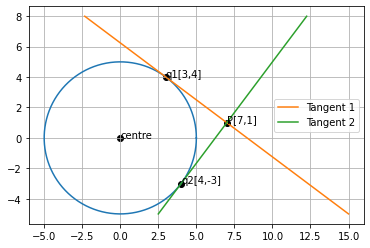
\includegraphics[width=\columnwidth]{fig_A_3.png}
   \caption{The plot of tangents to the circle }
\end{figure}

\end{document}
